\documentclass[10pt,a4paper]{article}
\usepackage[T1]{fontenc}\usepackage[utf8]{inputenc}\usepackage[spanish]{babel}
\usepackage{lmodern,geometry,graphicx,booktabs,hyperref}\geometry{margin=1.8cm}
\setlength{\parindent}{0pt}\setlength{\parskip}{6pt}\setlength{\emergencystretch}{3em}
\hypersetup{pdftitle={Proyecto 4: testbench del ZIP de practica},pdfauthor={Cristian Acevedo; Guillermo Arriaza; Eduardo Ponce}}
\begin{document}
\begin{center}{\LARGE Proyecto 4 -- Prueba del ZIP de práctica}\\[6pt]
Cristian Acevedo -- Guillermo Arriaza -- Eduardo Ponce\end{center}
\textbf{Entrada:} \path{Proyecto_4_Series_Practica_export.zip}. Nueva ejecución del procesador,
SPI y firmware activos, leyendo los precios exactos del ZIP sin normalización.
Los CSV son idénticos a las ocho series conocidas; esta repetición no es una
prueba fuera de muestra. Cada caso comienza con \$10\,000 y cero acciones.
Se cobra \$5 por orden ejecutada y se comprueba cada tick frente al modelo.

\textbf{Resultado:} 8/8 PASS; 160,000 ticks; 0 discrepancias; 98 compras y 92 ventas. Cadencia: 100 microsegundos. 
\textbf{Máximo observado:} 20.72 microsegundos; margen conservador 69.54 microsegundos.


\begin{center}\scriptsize\begin{tabular}{lrrrrrr}\toprule
Serie & Trader & Mantener & Compras & Ventas & DD (\%) & Primera compra \\\midrule
practica\_amd\_2022\_ene & 10738 & 8315 & 14 & 13 & 42.20 & 257 \\
practica\_amd\_2022\_may & 8540 & 9647 & 9 & 8 & 30.01 & 385 \\
practica\_apple\_2022 & 14263 & 11063 & 19 & 19 & 38.82 & 385 \\
practica\_apple\_2023 & 9272 & 10371 & 14 & 12 & 40.41 & 513 \\
practica\_meta\_2022 & 12836 & 9695 & 5 & 5 & 28.13 & 385 \\
practica\_netflix\_2022 & 10346 & 9179 & 15 & 15 & 46.72 & 257 \\
practica\_netflix\_2023 & 12432 & 9170 & 14 & 12 & 50.55 & 2177 \\
practica\_tesla\_2022 & 9342 & 9995 & 8 & 8 & 48.52 & 257 \\
\bottomrule\end{tabular}\end{center}
La estrategia supera a mantener en 5/8 series.
PASS indica coincidencia técnica, no rentabilidad. Los gráficos se calculan a
partir de las trazas RTL de esta ejecución. Los marcadores son operaciones
ejecutadas al precio siguiente al de la señal; los ticks empiezan en cero.

\textbf{Comportamiento.} SUM10 se revisa cada 128 ticks con umbral de 5\%.
Empieza en caja; la primera ejecución posible es en tick 257 y puede tardar más.
En Netflix 2023 ocurre en tick 2177: 21,77 segundos si la maestra usa 10 ms.
D4 apagado antes de una señal es esperable. Se verifican registros CPU,
STATUS/PRICE/SUM10/READY/DECISION, recepción única, reinicio y plazo de respuesta.

\textbf{Alcance.} Verilator simula en dos estados y complementa las pruebas
Icarus previas. Esta ejecución no lee la flash ni recibe telemetría física.
\par\smallskip\textbf{BIN SHA-256}\par
{\small\ttfamily 1f514301f1a7300351f4d3d8f48b77c2c85dcd2a274f44910d11d00df406db45}\par
\path{resumen.json} conserva hashes de ZIP, fuentes y trazas comprimidas.
\clearpage\subsection*{practica\_amd\_2022\_ene}
\begin{center}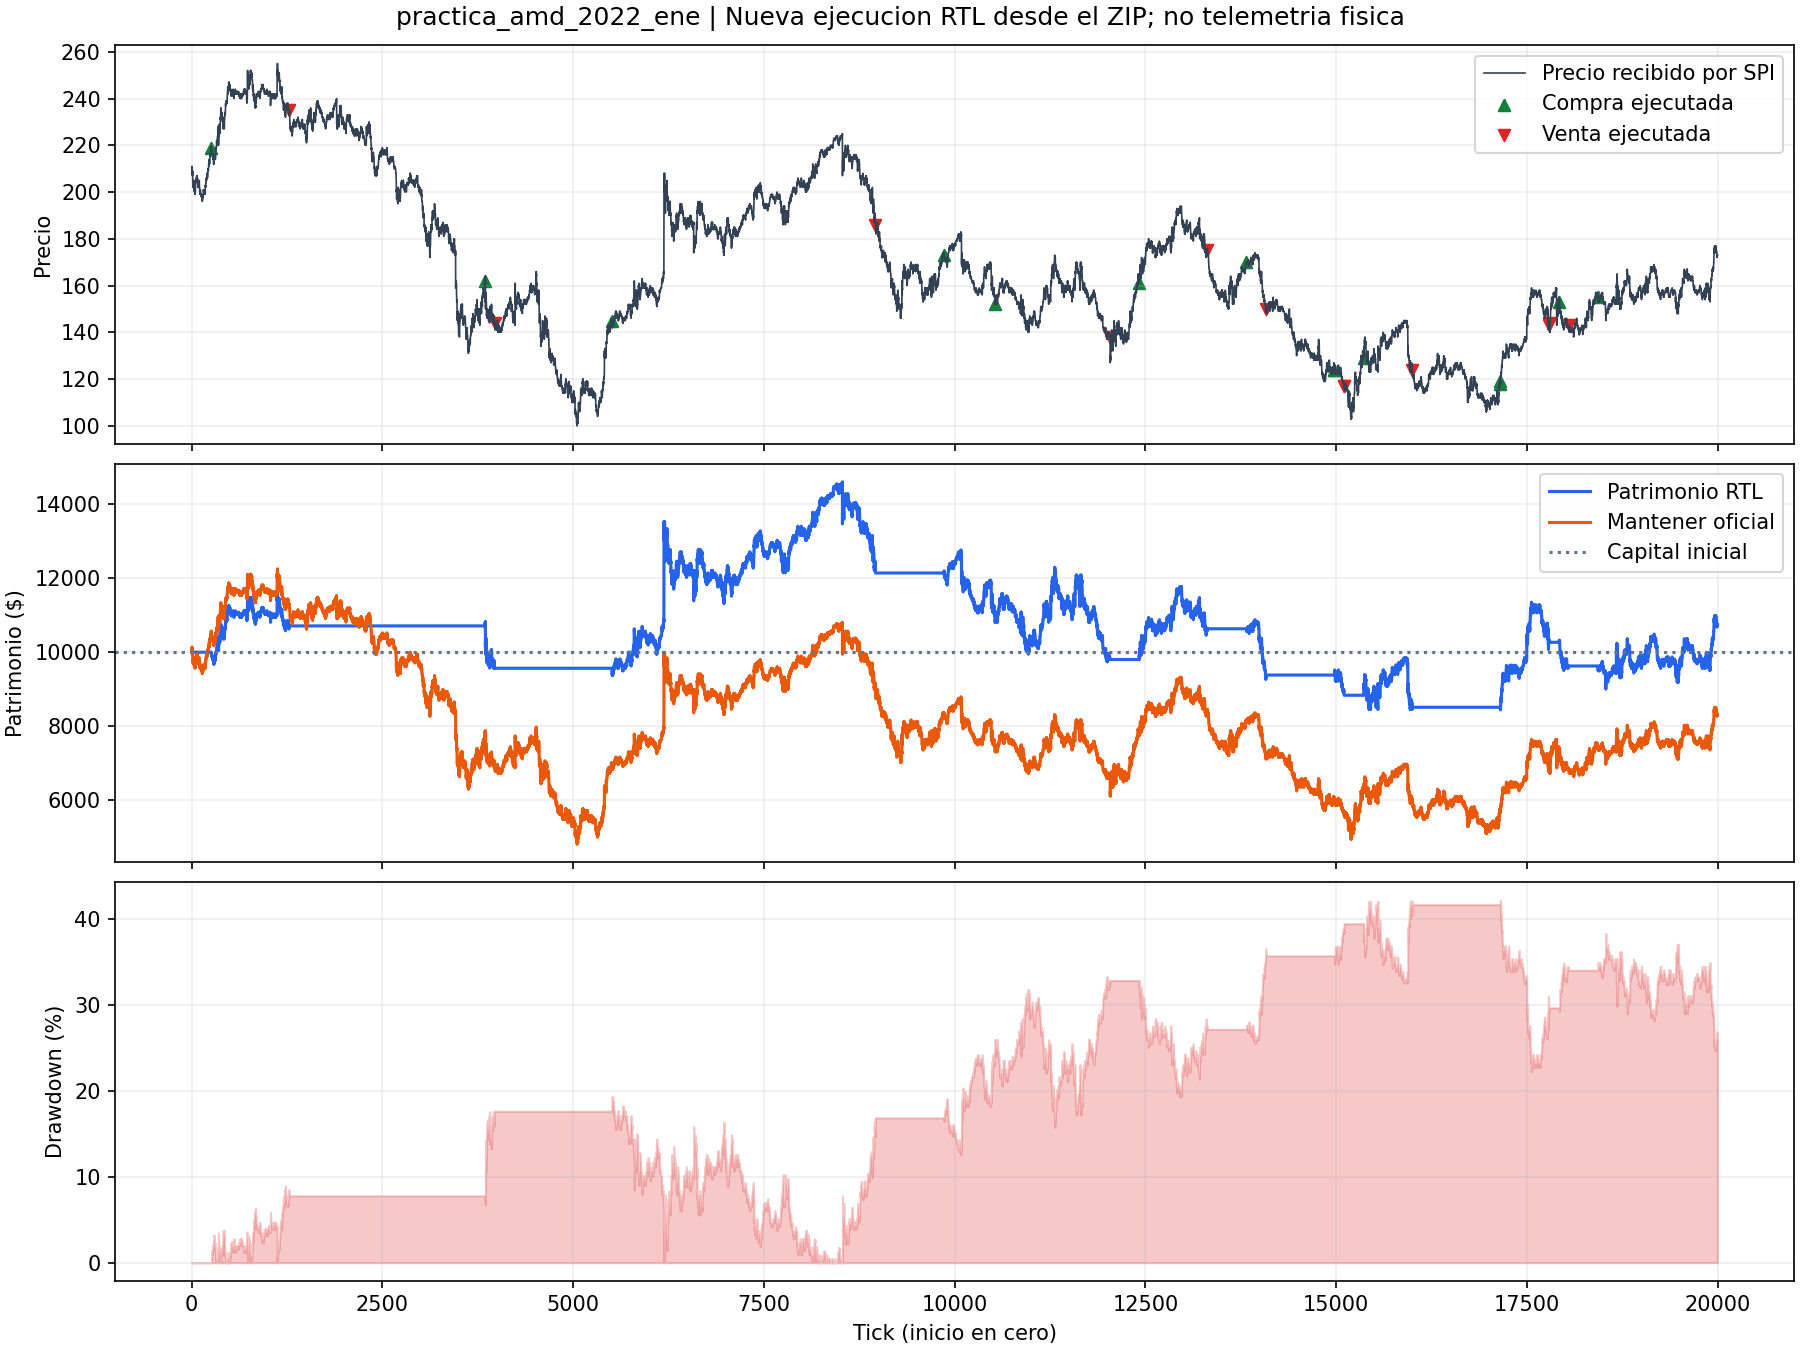
\includegraphics[width=\linewidth,height=0.78\textheight,keepaspectratio]{graficos/practica_amd_2022_ene.png}\end{center}
Primera compra: tick 257; primera venta: tick 1281. Patrimonio final: \$10738; comisiones: \$135.

\clearpage\subsection*{practica\_amd\_2022\_may}
\begin{center}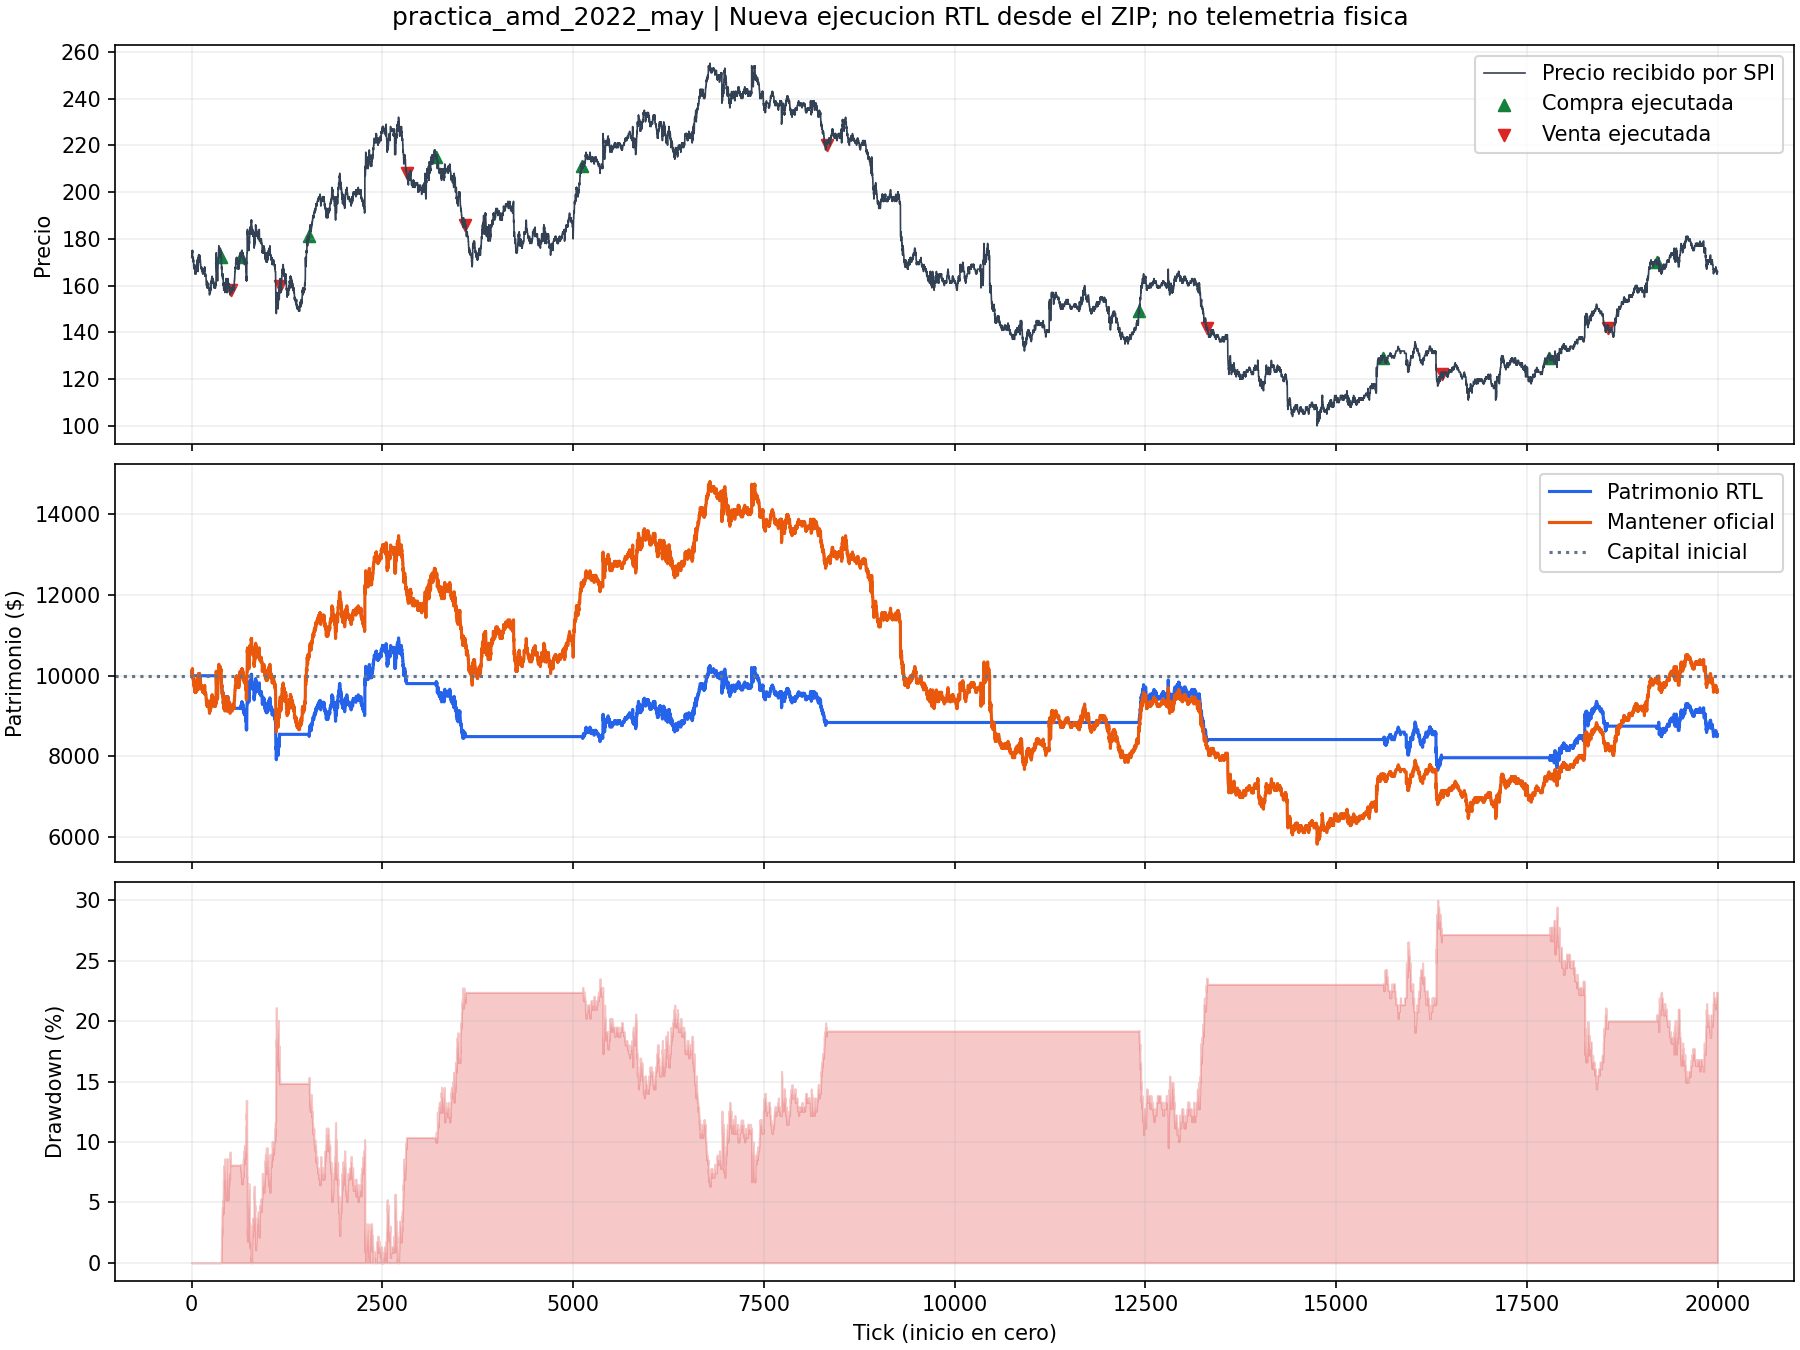
\includegraphics[width=\linewidth,height=0.78\textheight,keepaspectratio]{graficos/practica_amd_2022_may.png}\end{center}
Primera compra: tick 385; primera venta: tick 513. Patrimonio final: \$8540; comisiones: \$85.

\clearpage\subsection*{practica\_apple\_2022}
\begin{center}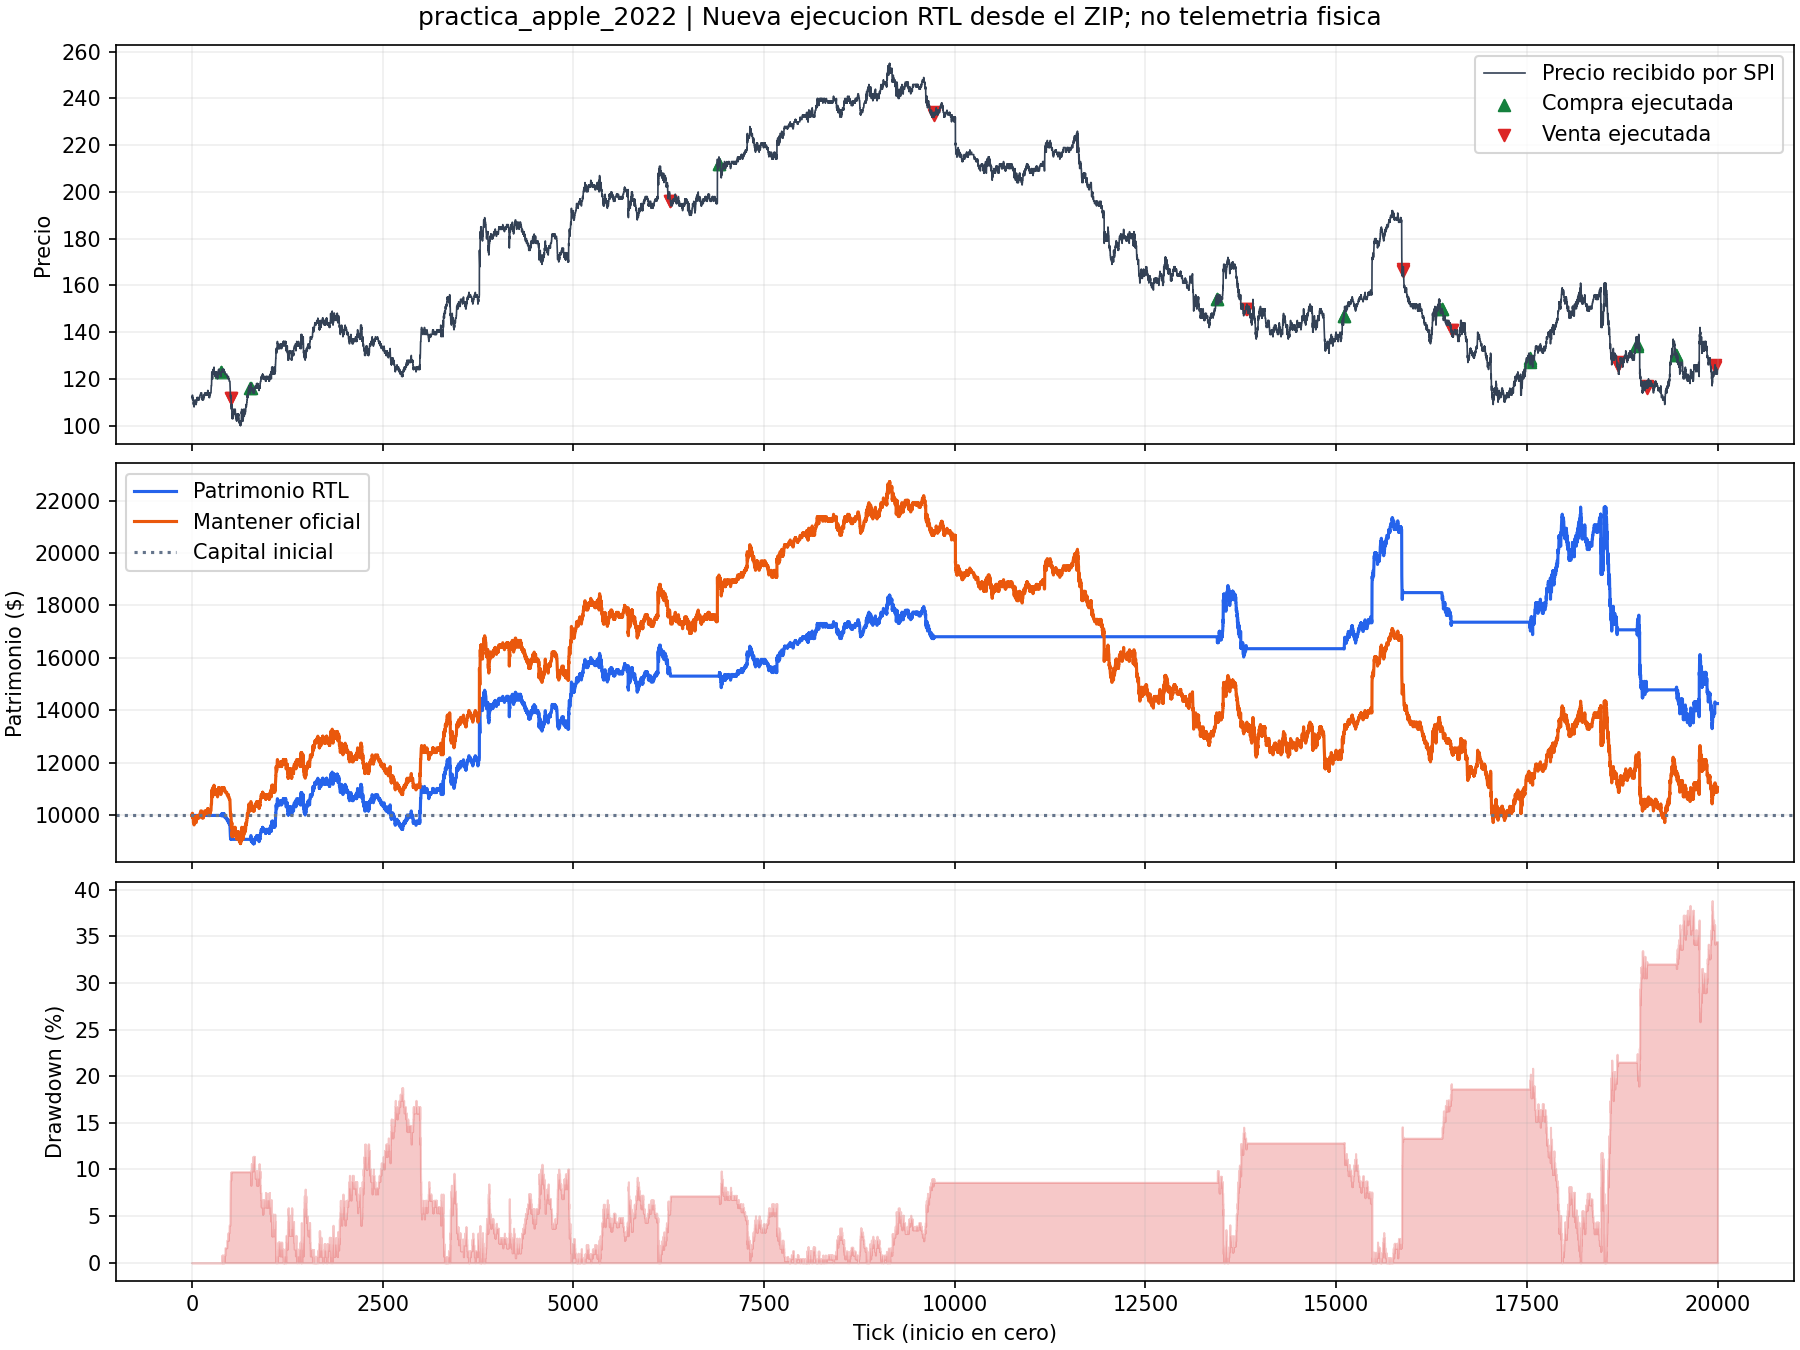
\includegraphics[width=\linewidth,height=0.78\textheight,keepaspectratio]{graficos/practica_apple_2022.png}\end{center}
Primera compra: tick 385; primera venta: tick 513. Patrimonio final: \$14263; comisiones: \$190.

\clearpage\subsection*{practica\_apple\_2023}
\begin{center}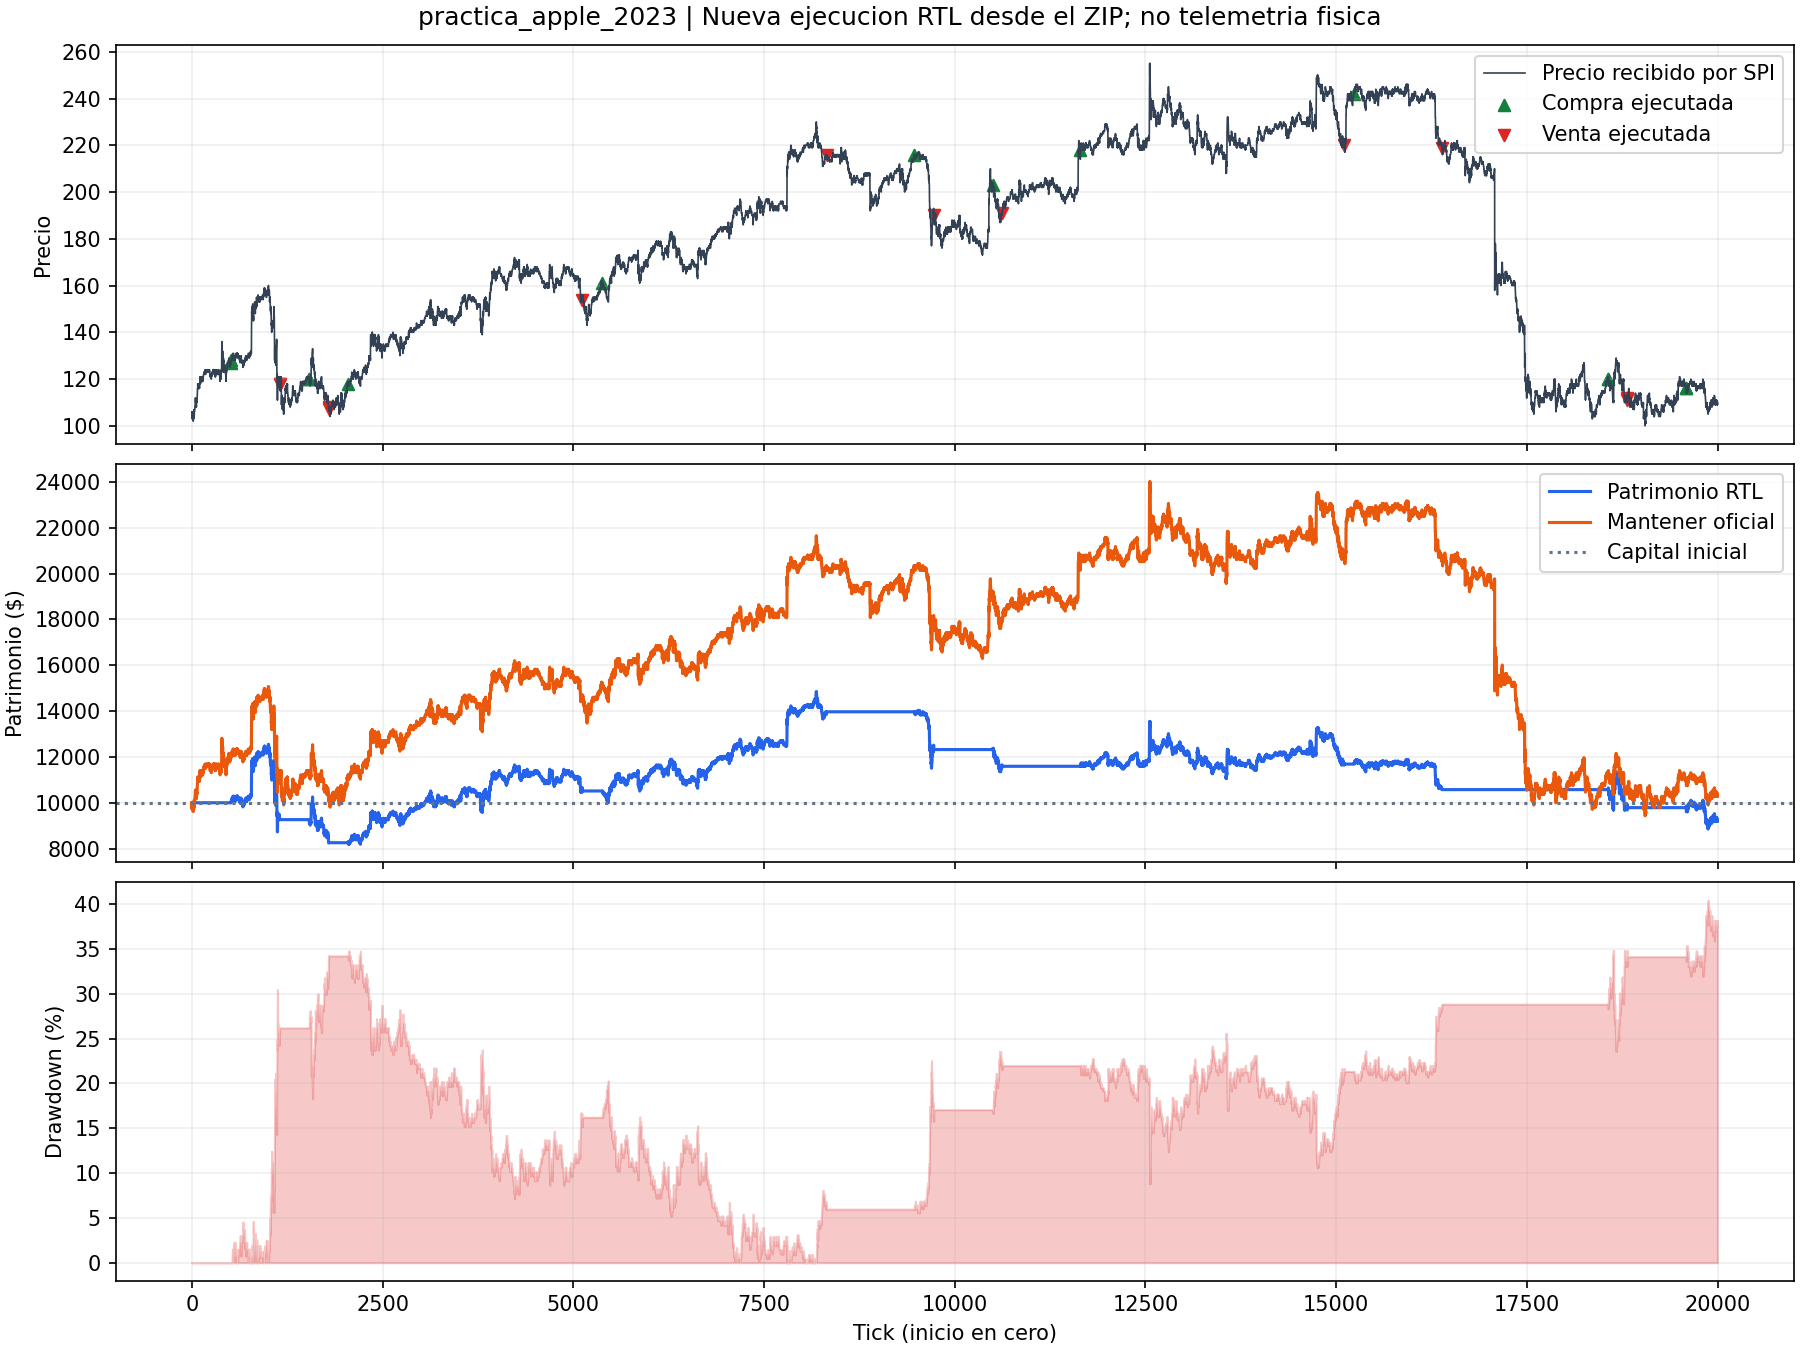
\includegraphics[width=\linewidth,height=0.78\textheight,keepaspectratio]{graficos/practica_apple_2023.png}\end{center}
Primera compra: tick 513; primera venta: tick 1153. Patrimonio final: \$9272; comisiones: \$130.

\clearpage\subsection*{practica\_meta\_2022}
\begin{center}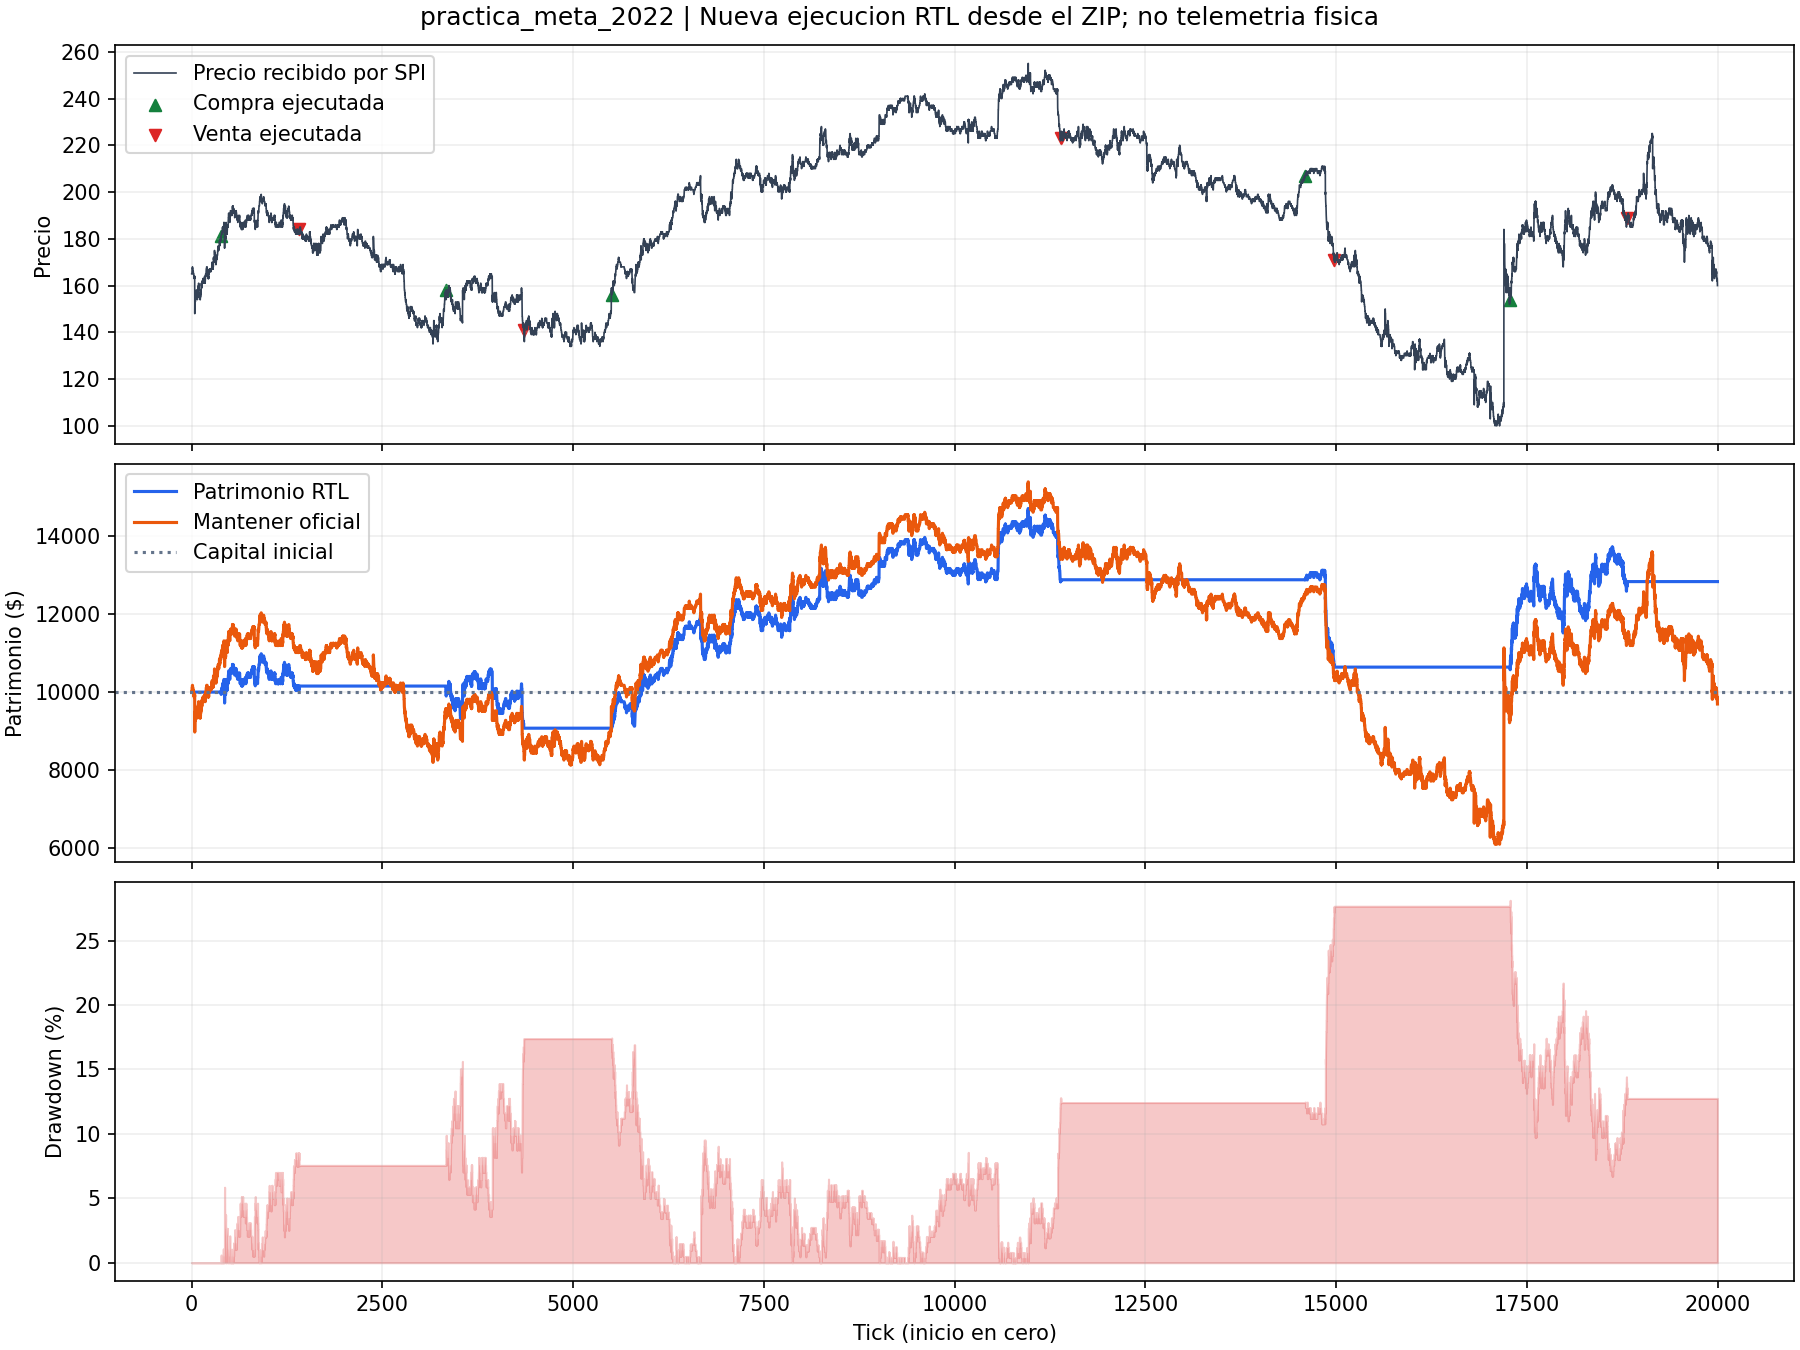
\includegraphics[width=\linewidth,height=0.78\textheight,keepaspectratio]{graficos/practica_meta_2022.png}\end{center}
Primera compra: tick 385; primera venta: tick 1409. Patrimonio final: \$12836; comisiones: \$50.

\clearpage\subsection*{practica\_netflix\_2022}
\begin{center}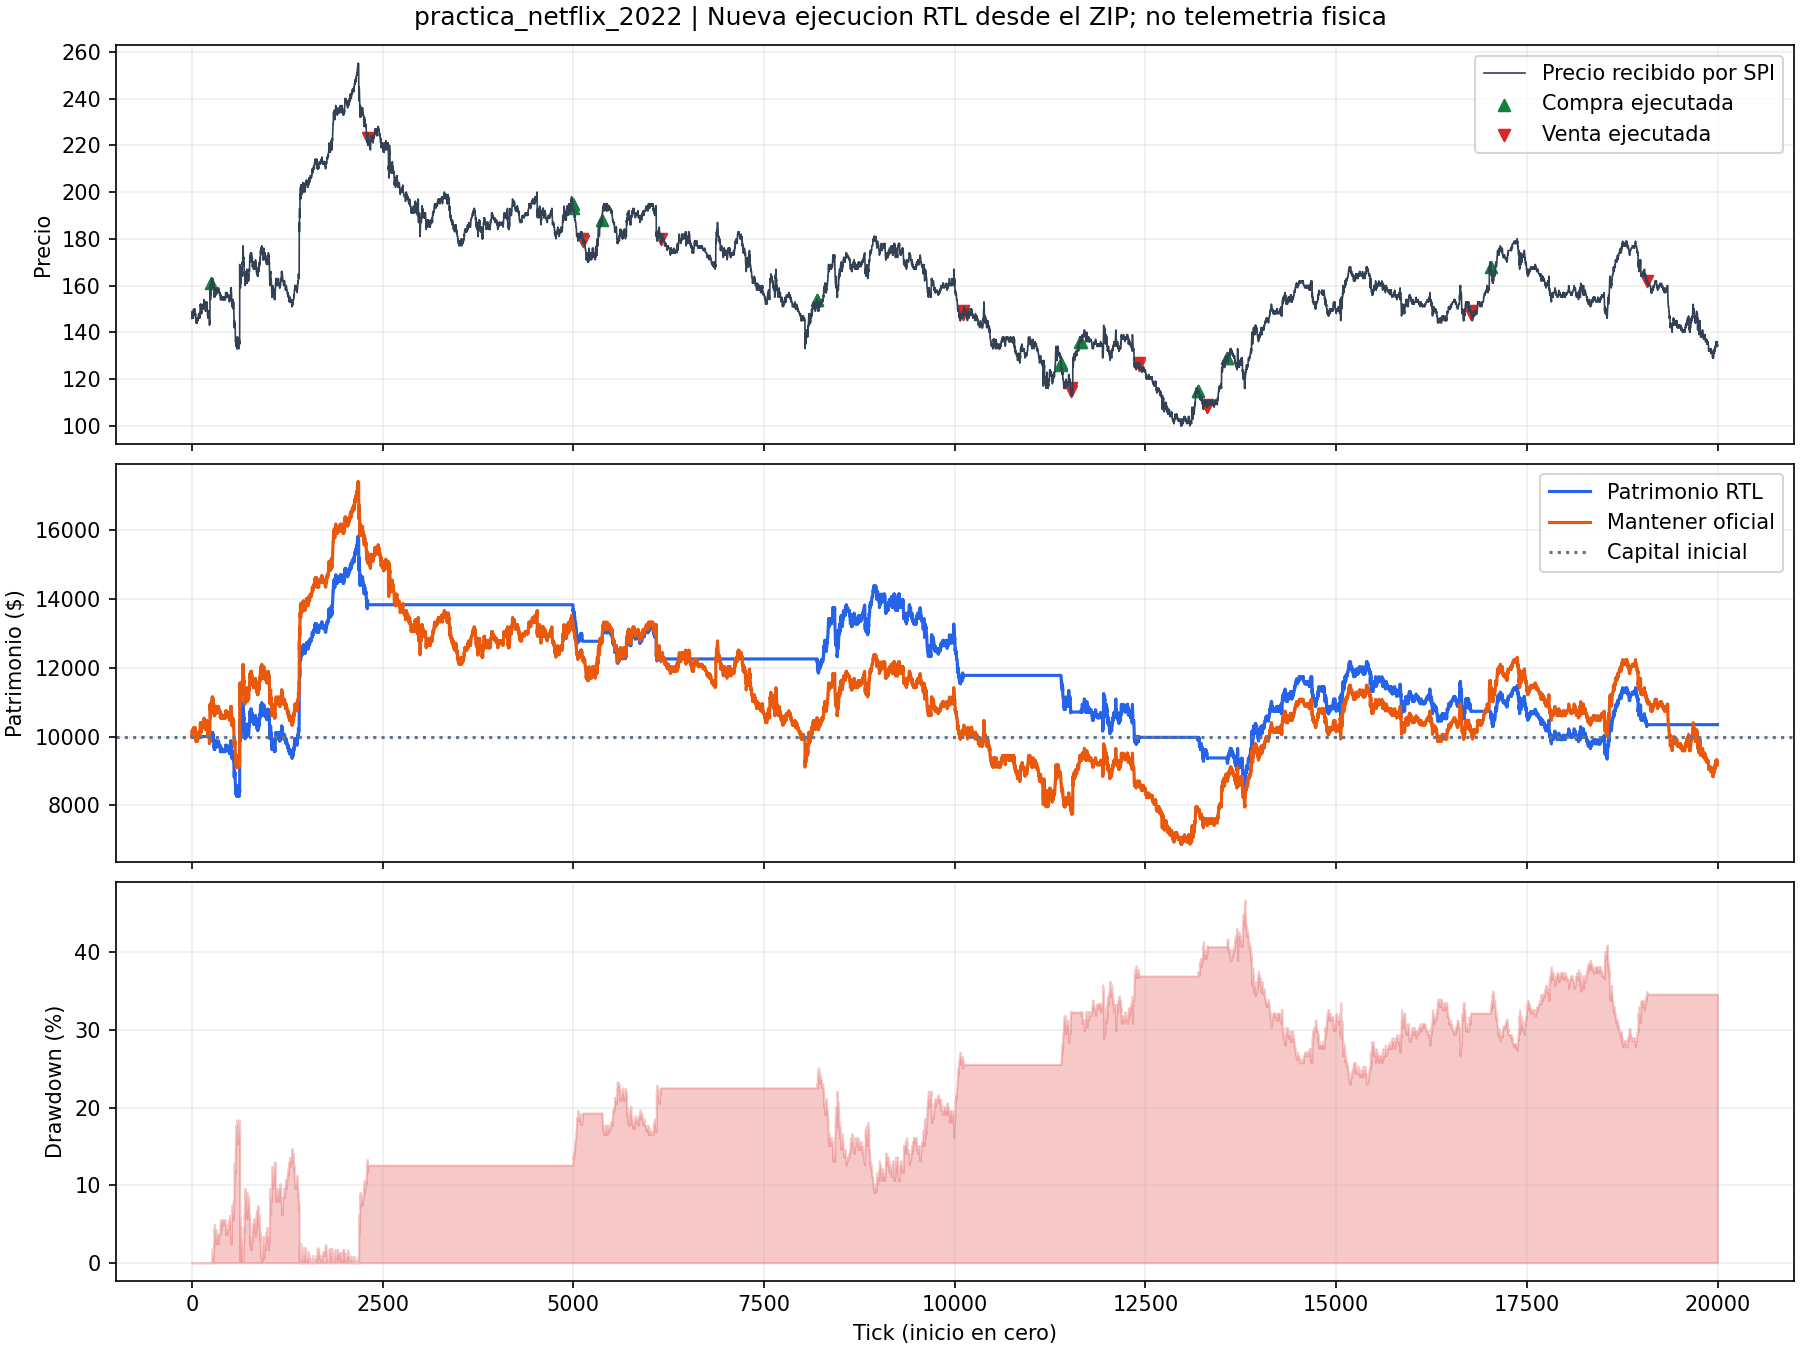
\includegraphics[width=\linewidth,height=0.78\textheight,keepaspectratio]{graficos/practica_netflix_2022.png}\end{center}
Primera compra: tick 257; primera venta: tick 2305. Patrimonio final: \$10346; comisiones: \$150.

\clearpage\subsection*{practica\_netflix\_2023}
\begin{center}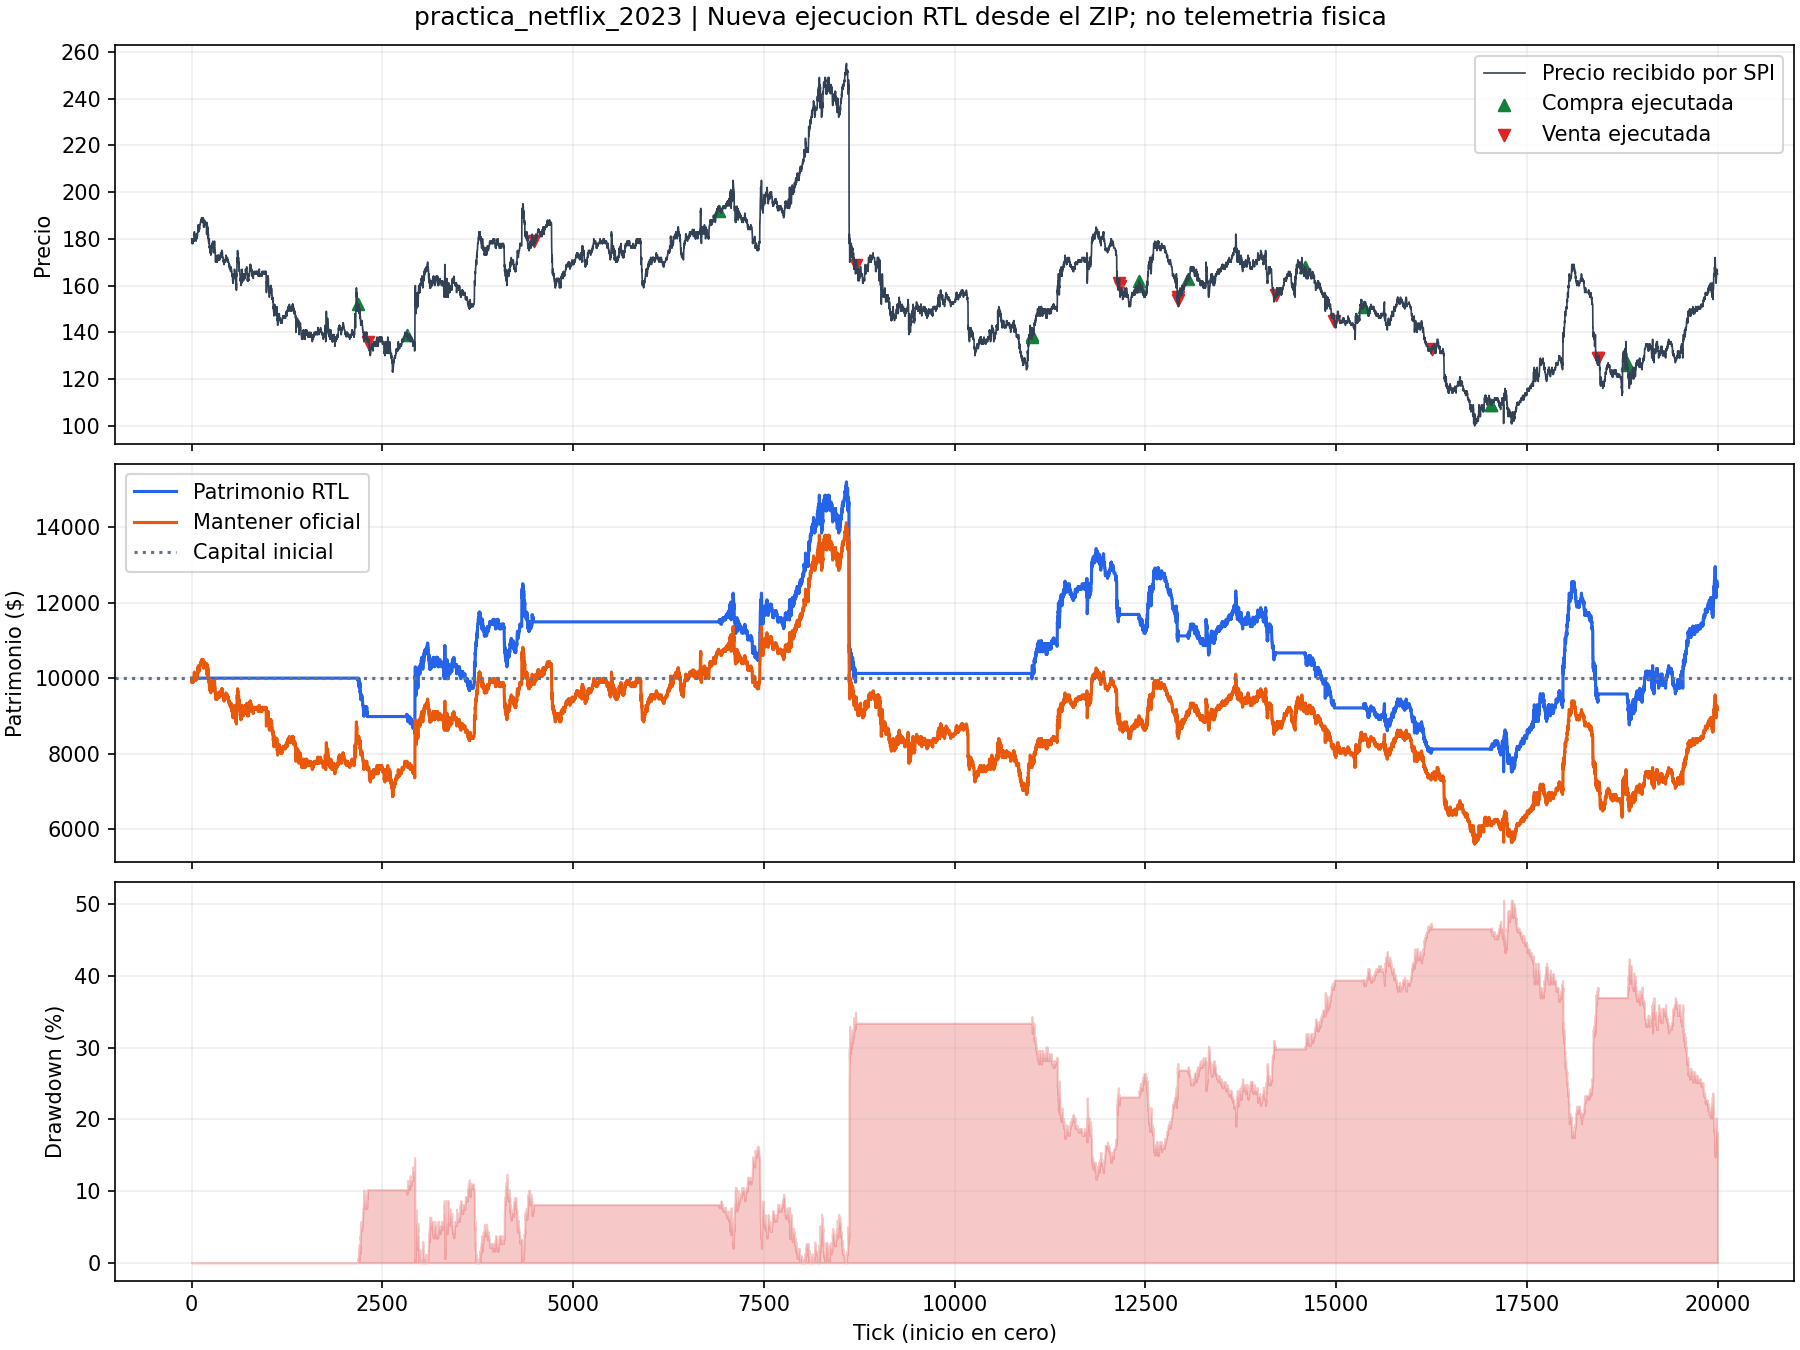
\includegraphics[width=\linewidth,height=0.78\textheight,keepaspectratio]{graficos/practica_netflix_2023.png}\end{center}
Primera compra: tick 2177; primera venta: tick 2305. Patrimonio final: \$12432; comisiones: \$130.

\clearpage\subsection*{practica\_tesla\_2022}
\begin{center}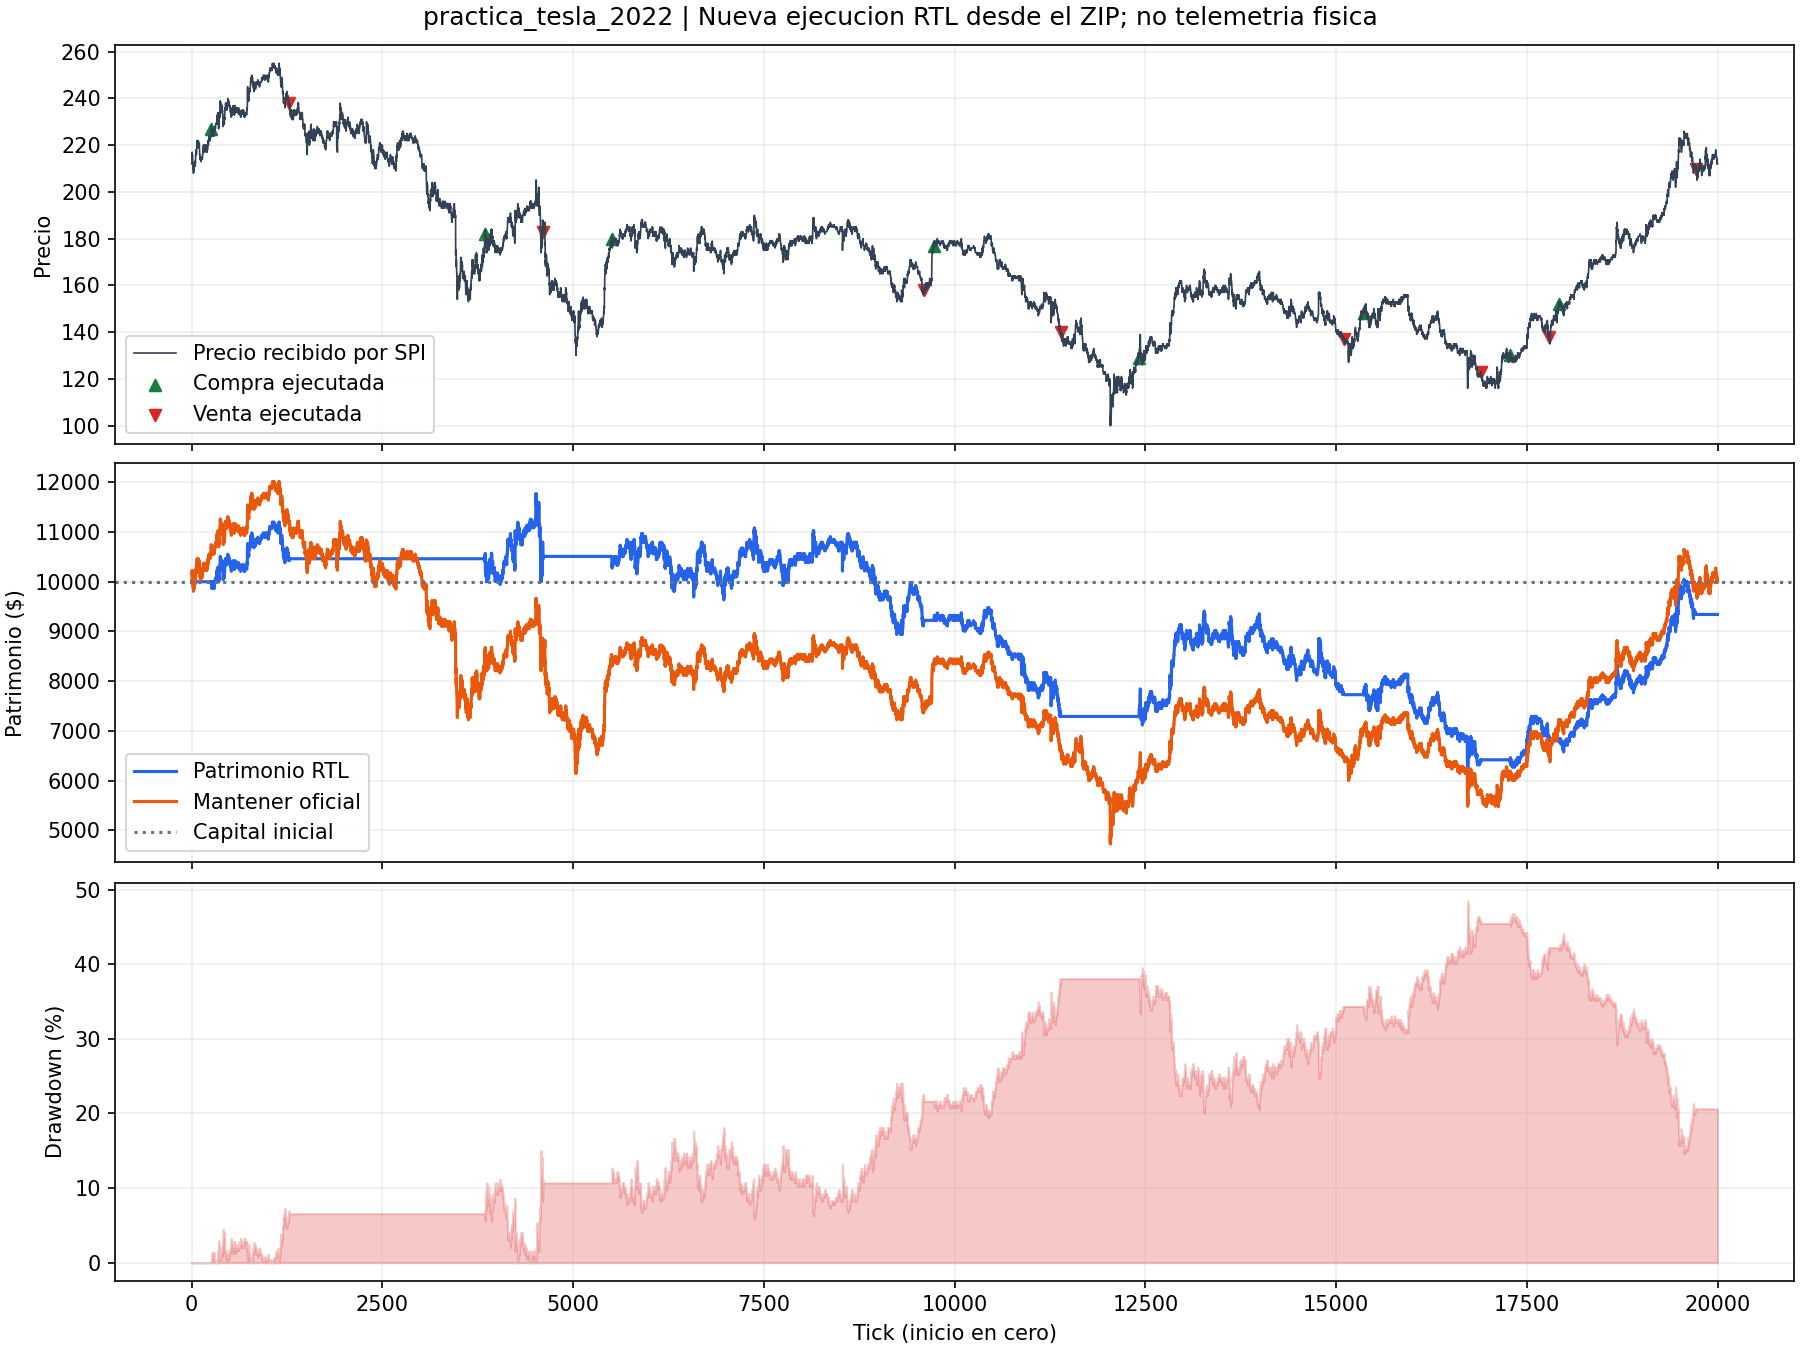
\includegraphics[width=\linewidth,height=0.78\textheight,keepaspectratio]{graficos/practica_tesla_2022.png}\end{center}
Primera compra: tick 257; primera venta: tick 1281. Patrimonio final: \$9342; comisiones: \$80.
\end{document}